

\chapter{Search by Object Location}
\label{ch:object_location}

The first representation technique we test search based on a visual description of the scene. For example, a user can recall the scene, i.e., he took a video of her family with the mountains in the background. The specific scene we search for was previously seen (memorized), and we look for a match in the database. This approach corresponds to the usual visual memory abilities - naming the objects and where they are located. We focus on retrieving similar scenes based on the image collage. The collage consists of several images places on the canvas. The position of the images corresponds to the position in the searched scene (see an example in figure \ref{fig:query_collage_comparison}).

\begin{figure}
\centering

\begin{subfigure}[t]{0.45\textwidth}
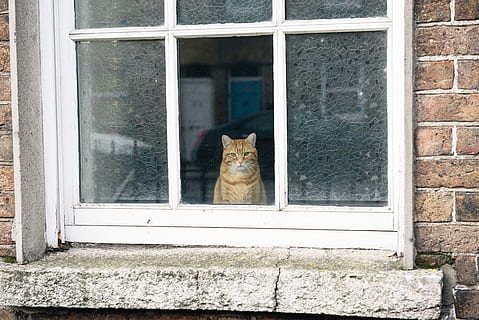
\includegraphics[width=0.9\linewidth]{img/cat_on_window} 
\caption{Query}
\label{fig:searched_scene}
\end{subfigure}
\begin{subfigure}[t]{0.45\textwidth}
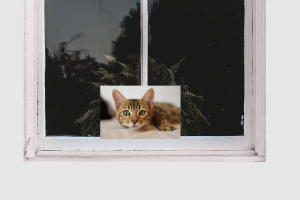
\includegraphics[width=0.9\linewidth]{img/cat_on_window_collage}
\caption{One of the possible collage description for the query}
\label{fig:collage_example}
\end{subfigure}

\caption{Example of searched scene (query) with possible visual description by a collage.}
\label{fig:query_collage_comparison}
\end{figure}

One of the alternative approaches could be using a word representation of the objects instead of images. Our approach aims to avoid the limitations of vocabulary size for word annotation. We believe that visually we can capture more diversity in the objects. Words often either omit more specific information about the look or are hard to obtain by annotation systems. For example, a single word for a human may represent a visually wide range of possibilities, based on clothes, age, and other attributes. We aim to avoid this bottleneck, and we proceed with the search based visual similarities.

In this chapter we utilise approaches based on two key information: 1. spatial information of the objects in the scene and 2. visual representation. Formally, representation $\hat{Q}$ of a query $Q$ is a set of pairs -- image and position. $\hat{Q} = \{ (pos_1, img_1), (pos_2, img_2), \dots \}$.

This chapter includes evaluations of the models on annotated collages. For more information about the dataset check the chapter \ref{ch:TODO}. 

\section{User-program interaction}

The query is a collage of one or multiple images. Each image also includes its relative position in the canvas (i.e. how far it is from top left corner relative to the size of the canvas).

The user interacts with the environment by adding, scaling, and/or moving images. Interactively, the closest representatives found in the dataset are returned. The user can select the final image, if they think they found the corresponding scene. 

The figure \ref{fig:query_collage_comparison} shows an example of the query. The goal is to be able to use any of the currently available image search engines to create a collage. The user places multiple images onto the canvas. Their position on the canvas is recorded and later used to target the database in regard to their position. 

\section{Features extraction strategies}

\subsection{Baseline -- Whole image representation}

Firstly, we introduce a baseline for our further experiments. In this case, we will ignore the information about the position of the objects. This leads to computing the representation of the items in the dataset.

\begin{figure}
\centering
\begin{boxedverbatim}
Database:
    - image: 1 feature vector (1 Dimensional)
    - model M
Query:
    - query_images: feature vectors from M
    - compared to: each image in the database
\end{boxedverbatim}
\caption{Overview of the Whole Image approach}
\end{figure}

\subsection{Splitting an Image into Regions}

% In our first approach we cut the image into fixed regions. We aim to capture the 
% representation of each of these regions. This offers us an information specific for each region.

% With the query we can compare the features representation of the query and of the particular regions we are interested in.

% Image
% - Split to nxm regions
% - Compute deep representation for each of the regions

% Query
% compute deep representation for the image in the query
% for each image in the database, compare this representation to the representation of the region with highest IoU

% In our first approach we split the image to a regions. We compute a deep representation using neural network for each region and the whole image. 

One of the natural ways to capture spatial information about the objects in the scene is to cut the images into fixed regions. We then can capture visual information for these regions separately. For the incoming queries, we may compare the visual information of the query only to the regions which collide in the zone of the interest.

We split each image  $img \in D$ in the database into $N \times M$ regions. To provide full information about the image, we make an requirement for the regions to cover the whole image. To preserve square shape of the regions and also an option to obtain more information, we allow overlaps between the regions. For each of the newly region $r_{img, i, j}$ we preserve information about its original image $img$, region’s position (coordinates of the region $i, j$) and visual features $f(r_{img, i,j}$.

\begin{figure}
\centering
\begin{boxedverbatim}
Database:
    - image:
        - Multiple Crops:
            - coordinates
            - feature vector (1 Dimensional)
    - model M
Query:
    - query_images: features vectors from M
    - compared to: only to related crops from each image
\end{boxedverbatim}
\caption{Overview of the Regions' approach}
\end{figure}



% \section{ Using Deep Representation}
%   - Using Deep Representation
%       = Using antepenultimate layer of classification networks

% \section{Multi-query search}
% - Multi query search
%   - Fusion methods
%   - Comparison of both approaches with multimodal performance over different fusion techniques

% Our work focuses on difficult to describe scenes with multiple easy to recognize objects. In this questions a natural question of how to rank the results based on multi query.

% In this section we go through several approaches we tested. We base our 

% \subsection{Fusion Methods}

% \section{Evaluation}
% In this chapter we evaluate all previously mentioned approached. Firstly, we describe our methodology behind the experiments and then we proceed through all approaches. 

\subsubsection{Regions Shape}

In order to use transfer learning for common CNN and to avoid additional skewing in resizing, we limit to the regions only to the shape of squares. Since this input size of the square is one of the parameters, we aim to use the size of the squares the same as the size of the input of the network. This helps us to avoid unnecessary scaling which may be introduced when the length of the side of the square does not match with the input for the network.

With fixed-width $w$ of the square and the number of regions $N \times M$, we define the following regions:
\[ 
r_{i,j} = {(( \text{image\_height} - w) / (n - 1) *i, ( \text{image\_width} - w) / (m - 1) * j)}
\]

With the condition on full coverage of the image (i.e. \(w n >= \text{image\_height}\), and for $m$ respectively) we obtain full coverage of the image by the regions. Overlaps are evenly distributed over both axis.

\begin{figure}
\centering
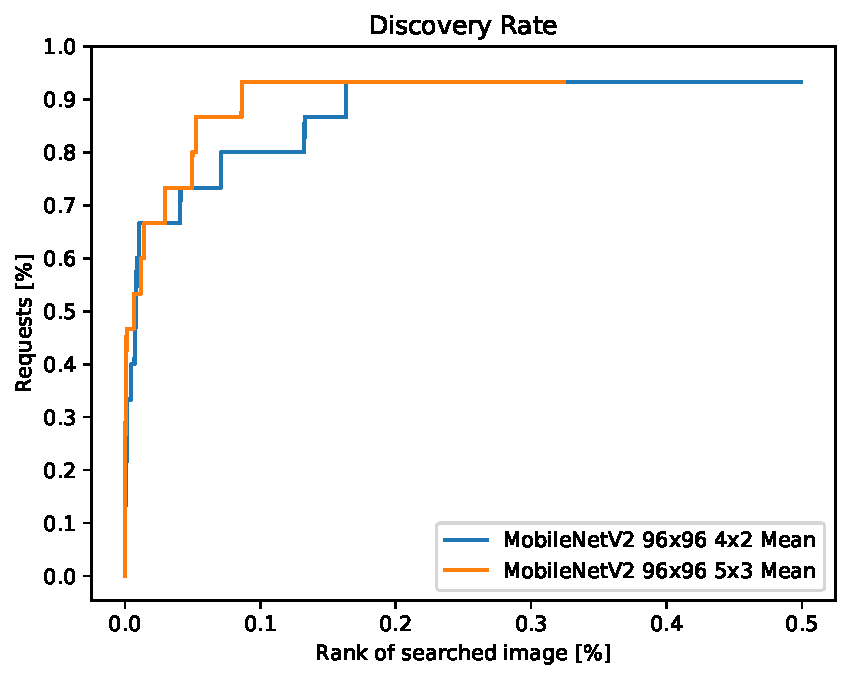
\includegraphics[width=\textwidth]{graphs/78f2a977489ac08dddac6f53446b388292306ec95f9dcbc7ca8359fbedfed9b0}
\caption{Performance of the system based on different number of regions per image}
\label{fig:different_number_regions}
\end{figure}

\subsubsection{Choice of regions}

Given one incoming query image with its position and shape we propose several methods for choice of the “targeted” regions. For each one of the fixed regions we compute %\[\text{IoU_{i,j,k}} = \text{IoU}(Ri,j; Qk) for all i, j. \]

First of the options, is to only compare the region with highest Intersection over Union, limiting to the argmax IoUijk. I.e. for each i belongs I only one region would taken into account.

Second approach is to collect all intercepted regions for the similarity. This is an exhaustive process. This may result in increased computation time, i.e. usually from 2 to 9 times slower. In case of a huge set of data without any indexing, it may increase time of a request from 1 sec up to several seconds.

Third choice is to limit the number of targeted regions to a certain number. This offers us an advantage of fuller coverage and possibility for better match in neighbouring region, on the other hand provides an upper bound for the computational time required per request. 

Visualisation of chosing different number of crops can be seen in figure \ref{fig:fish_with_grid}. A comparison of the performance dependend on different number of chosen crops is shown in figure \ref{fig:crop_limitation}.

\begin{figure}
\centering
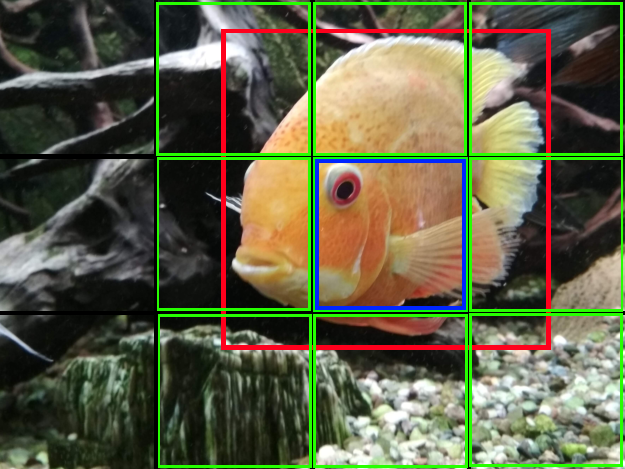
\includegraphics[width=0.6\textwidth]{img/fish_grid_regions}
\caption{Example of choosing the corresponding regions. Red: query position; Green: all intercepted regions; Blue: region with highest IoU.}
\label{fig:fish_with_grid}
\end{figure}


\begin{figure}
\centering
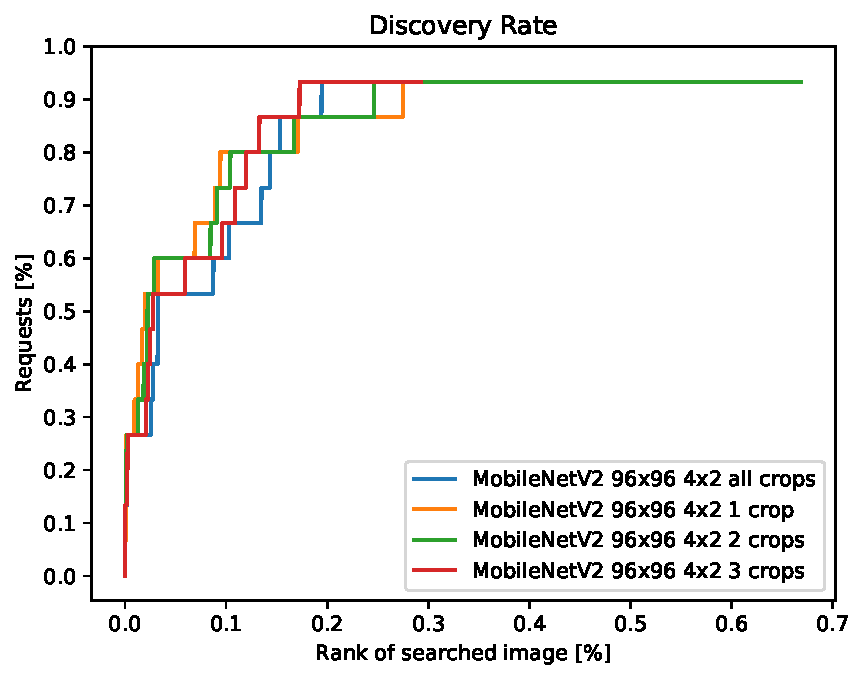
\includegraphics[width=\textwidth]{graphs/c2cf4e147040018e6cfc46043bb59de4f5f3e83441c1e1024af0b7bab644a994}
\caption{Performance of the system based on different number of chosen crops}
\label{fig:crop_limitation}
\end{figure}


\subsection{Using more information from antepenultimate layers from CNN}

The previously mentioned approach has a shortcoming. It is not able to grasp the arbitrary position of the object, rather it has limitations to previously fixed regions. This may lead to decreased performance for the objects, which cover a bigger part of the scene, i.e. in the previous case, it may overlap over multiple regions. This brings not only computational disadvantages but also reduces the amount of information which are used when compared to the query.

We propose an approach, where an antepenultimate layer of common CNN's may be used. Common CNNs are built out of several building blocks, i.e. convolution layers intervened by pooling (TODO image). This approach proved its ability for image recognition and many other related tasks (TODO add source). Many of the current state-of-the-art models use the pooling layer before fully connected layer for categorization.

We aim to leverage this antepenultimate layer, which contains not only visual features but also spatial information.

\begin{figure}
\centering
\begin{boxedverbatim}
Database:
    - image:
        - feature vector (3 Dimensional):
    - model M
Query:
    - query_images: features vectors from M, then average pool)
    - compared to: average pool over selected region for item 
                   in the database
\end{boxedverbatim}
\caption{Overview of the Spatial approach}
\end{figure}


\subsubsection{Choosing region of interest in the layer}

Layers before pooling on which we focus are 3 dimensional. First two dimensions contain spatial information, which is propagated from the previous layers. The third dimension contains visual information.

In order to obtain only a part of this layer we are interested in (i.e. our query was placed in that specific region) we need to take only a subset over first two dimensions. For a query defined by Qi = (y, x, h, w) and layer Li with first two dimensions H, W we consider a Li[y * H, x*W, (y+h) * H, (x + w) * W]. 

It is important to notice, that these layers use to have significantly lower height and width, compared to the input of the network. For example, before-last-pooling layer of Resnet50V2 has dimensions (7,7,2048). Therefore, we round our subset to nearest whole number and in case of no intersection we maintain at least intersection of size 1x1.

After this choice of the region of interest, we continue with the pooling layer in order to obtain one feature vector.

In comparison with the previous Splitting in regions approach, we see an enhanced ability to grasp more variability in object position. Especially, in queries which overlap most of the regions. On the contrary, this approach may require more memory, as for comparison for Resnet50V2 with 12 regions we needed to work only with 12 feature vectors. With the before-last-pooling layer we need for Resnet50V2 to work with 49 feature vectors. This may not be limitation with smaller feature vectors, but may come as a practical limitation based on the size of the dataset and computability power available.


\section{Ranking}
In the previous sections, we talked about the obtaining feature vector for the items in the database of the regions we are interested in. In this section, we take a closer look on further processing these obtained feature vectors.

Assuming we have an image for the query, we use the same model to compute the feature vector as was used to precompute the features for the database. Based on that we define a distance D, as the distance between the feature vector of the query and feature vector of the item in the database. This comparison to each database item gives us the distance between each item in the database and our query image.

Based on these distances we order the results, starting from the lowest to the highest distance. This distance acts as an inverse for the similarity. Similar to the results are, lower is the distance.

We use 3 main distance metrics:
Cosine Distance
Euclidean L2 distance
Euclidean L1 distance

\section{Multiple objects in the scene}

So far we talked only about handling queries consisting of one searched object. This limitation is very strict and therefore we experiment with multiple approaches to index the database based on multiple objects in the scene.

Firstly we make an assumption, that all query images have the same importance and are expected to be with the same level of relevance. Therefore we approach this problem as a set of query images, rather than as an ordered list.

We work further only with already precomputed rankings with corresponding distances for each image/part of the image. We propose several ways to merge the rankings.

We define ranking $R$ as a set of distances between the query image $q$ and database item $i$. We look for a function $r: R^n \rightarrow R$, which merges multiple rankings into one final ranking. Our goal is to minimize rank for each of the queries in the test items.

We tested several functions for this role and to compare a function that does not take into account the distances with different functions over the distances. A comparison for MobileNetV2 can be seen in figure \ref{fig:ranking_funcs}.

\begin{figure}
\centering
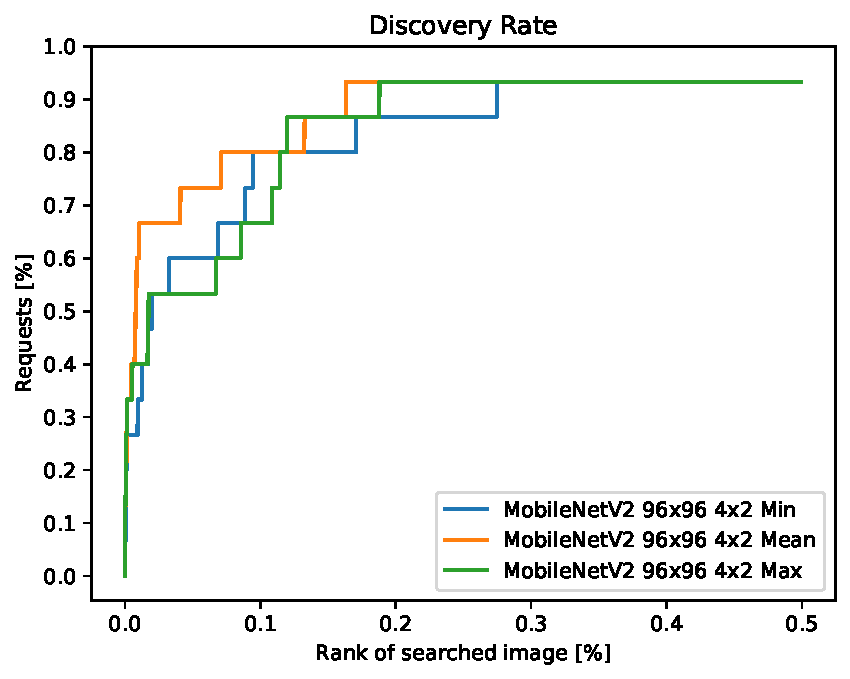
\includegraphics[width=\textwidth]{graphs/362cb9a687ce05c7732f973defca88fb8c5c393f5992066521343314698c9de7}
\caption{Performance of the system based on different fusion method}
\label{fig:ranking_funcs}
\end{figure}

\section{Padding}

Our input images provided by a user do not have to be a square images. Although, we need to prepropress these to obey the input shape of the feature extraction model we use. These models use usually square shaped input. In our case, we compare the performance of the solution based on three different approaches on input reshaping. We compare padding the input with black or white and our third option is rescaling the images. Rescaling is done in the manner, where distortion occurs for non square images, i.e, a tree becomes shorter and wider, and the car becomes narrower and taller. The results are available in the figure \ref{fig:TODO}

\section{Dimensionality reduction}

In the previous sections we evaluated several hyperparameters of the system to achieve the best performance. In this section we take a look in reducing the dimensionality of the extracted features. The extracted features from the neural networks with removed last fully connected layer are often high dimenisonality data (for MobileNetV2 its 1024 features, for Resnet50 it is 2048 features). Even though we were able to test the hyperparameters without introducing another factor -- dimensionality reduction -- we want to test also if such reduction can have also positive effects.

\todo[inline]{Mozno viac popisat PCA?}

We perform Principal Component Analysis on the extracted features. We evaluate the effects of the PCA given different number of extracted components. This helps us to significantly reduce the size of the dataset used and therefore offers us a solution with good scalability.

